This chapter presents an evaluation of \bpfbox{} and \bpfcontain{} in terms of their
performance and security. \Cref{s:eval-performance} presents the methodology and results
of a performance evaluation involving micro- and macro-benchmarking of \bpfbox{} and
\bpfcontain{}. Results are compared with AppArmor~\cite{cowan2000_apparmor}, a popular
\gls{lsm} framework for \gls{mac} security policy. Finally, \Cref{s:eval-security}
presents a security analysis of \bpfbox{} and \bpfcontain{} under the threat model
outlined in \Cref{s:cp-threat-model} of \Cref{c:confinement-problem}.

\section{Performance Evaluation}%
\label{s:eval-performance}

This section presents a performance evaluation of \bpfbox{} and \bpfcontain{}, measuring
their performance overhead using a variety of micro- and macro-benchmarking tests. In
particular, we leverage the Phoronix Test Suite~\cite{phoronix} to measure overhead across
a variety of computational tasks, workloads, and kernel interfaces. Each of these
benchmarks exercises a different subset of \bpfbox{} and \bpfcontain{}'s enforcement
engine, providing an approximation of their impact on the overall system. We also measure
the performance of the base system as a control, and the performance overhead of AppArmor
as a basis for direct comparison. The subsections that follow provide an overview of the
testing methodology and present the benchmark results.

\subsection{Methodology}%
\label{ss:eval-methodology}

As a test environment, we utilize a bare-metal system running Arch Linux with a stock
5.12.14-arch-1-1 kernel. The choice of a bare-metal system (rather than a virtual machine,
for instance) reduces the risk of introducing additional sources of variance into the
benchmarks. \Cref{tab:system-config} provides a detailed account of the test system
configuration.

\begin{table}[htp]
  \centering
  \footnotesize
  \caption[System configuration for benchmarking tests]{System configuration for benchmarking tests.}%
  \label{tab:system-config}
  \begin{tabular}{ll}
  \toprule
  Item & Description / Configuration \\
  \midrule
  CPU & Intel i7-10875H; 8 cores, 16 threads at 2.3GHz; 16MB cache\\
  GPU & Nvidia RTX 2060 with 6GB GDDR6 VRAM \\
  RAM & 2$\times$16GB DDR4 at 3.2GHz \\
  Disk & 1TiB Samsung NVME M.2 SSD \\
  \midrule
  \gls{os} & Arch Linux (Rolling) \\
  Kernel & Linux v5.12.14-arch-1-1 \\
  Libc & glibc v2.33-5 \\
  Phoronix & v10.4.0-1 \\
  \bottomrule
  \end{tabular}
\end{table}

To simulate the Docker container use case, we run all tests in a privileged Docker
container, using Docker volumes to mount the host filesystem in the benchmarking
directory. To improve benchmarking accuracy, we also perform the following setup before
each test. (1) We disable SMT hyperthreading by turning off each logical CPU core pair,
leaving only the physical cores active; (2) We disable turbo boost, capping the CPU at its
stock speed of 2.3GHz; (3) We set the CPU frequency scaling governor to
\enquote{performance} to limit the impact of thermal throttling and power saving features;
and (4) We globally disable \gls{aslr} by setting the appropriate kernel parameter. These
settings, consistent with best practices, improve benchmark accuracy by making the
environment more consistent and eliminating as many external factors as possible.

\begin{table}[htp]
  \centering
  \footnotesize
  \caption[List of benchmarking suites and what they measure]{
    A list of the benchmarking suites used to test performance overhead, and what each
    measures.
  }%
  \label{tab:suites}
  \begin{tabular}{llp{3in}}
  \toprule
  Test Suite & Test & Measures \\
  \midrule
  OSBench                    & Create Files       & Time to create and delete files \\
                             & Create Threads     & Time to create new threads \\
                             & Launch Programs    & Time to fork + execve \\
                             & Create Processes   & Time to create new processes \\
                             & Memory Allocations & Memory allocation throughput \\
  Kernel Compilation         & ---                & Time to compile Linux Kernel \\
  Apache Web Server          & ---                & Apache HTTP request throughput \\
  % \gls{ipc}                  & Unix Socket        & Unix socket throughput \\
  %                            & TCP Socket         & TCP socket throughput  \\
  %                            & Named Pipe         & Named pipe throughput  \\
  %                            & Unnamed Pipe       & Unnamed pipe throughput \\
  \bottomrule
  \end{tabular}
\end{table}

To measure the performance overhead of \bpfbox{} and \bpfcontain{} (compared with the base
system and with AppArmor) we leverage the Phoronix Test Suite~\cite{phoronix}, a popular
cross-platform benchmarking framework that has seen wide use for measuring system
performance. The Phoronix framework comprises a number of open source test suites, each
targeting a different aspect of system behaviour. For the purposes of this thesis, we
select three separate test suites, measuring a variety of \gls{os}-level functionality and
exercising multiple \gls{lsm} hooks. In particular, we select the OSBench suite, the
Kernel Compilation suite, and the Apache suite. \Cref{tab:suites} describes each test
suite and what it measures.

\begin{figure}[htp]
  \centering
  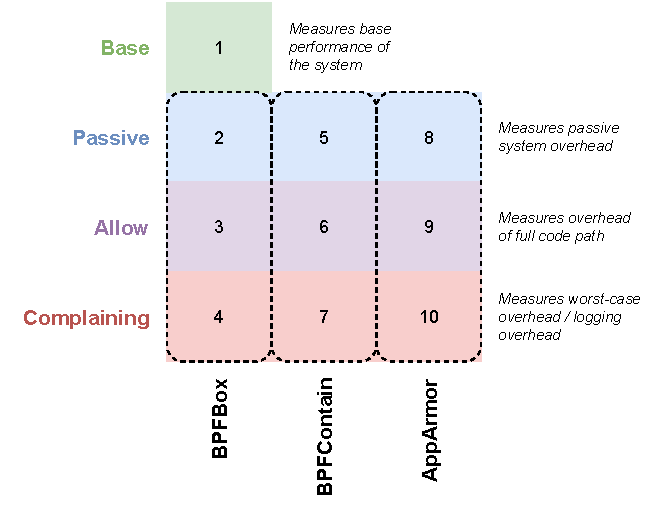
\includegraphics[width=0.8\linewidth]{figs/eval/configuration.pdf}
  \caption[Benchmarking system configurations]{
    The various system configurations used in the benchmarking tests.
  }%
  \label{fig:configuration}
\end{figure}

We consider ten system configurations in total (\Cref{fig:configuration}). The
\textbf{Base} configuration is the base system without any \glspl{lsm} or other
confinement primitives active or loaded in the kernel. The \textbf{\bpfbox},
\textbf{\bpfcontain}, and \textbf{AppArmor} configurations measure the performance
overhead of \bpfbox{}, \bpfcontain{}, and AppArmor, respectively. We then divide each of
these three configurations into three distinct test cases each. The \textbf{Passive} case
measures global system overhead without any active enforcement. The \textbf{Allow} case
measures active enforcement, allowing all security-sensitive operations. Finally, the
\textbf{Complain} case measures the worst-case overhead for each system, exercising the
full code path of each \gls{lsm} hook and logging every attempted access.

To ensure statistically valid results, we run each test at least eleven times, until
a standard deviation of at most $2\%$ of the mean is achieved. This is a sensible default
enforced by the Phoronix Test Suite to ensure statistically valid results. We also discard
the first run of each test to control for initial I/O transients. In total, the result is
at least ten trials for each test suite and system configuration. For reproducibility, we
make the benchmarking repository publicly available\footnote{Benchmarking tests are
available: \url{https://github.com/willfindlay/bpfcontain-benchmarks}}, including all
results and related scripts.

% \begin{inprogress}
%   \begin{itemize}
%     \item Test environment
%     \begin{itemize}
%       \item Describe system specs
%       \item To improve benchmark accuracy, we disable ...
%       \item We run tests in a privileged Docker container
%       \item Arch Linux Kernel 5.12.15-arch-1
%     \end{itemize}

%     \item Phoronix Test Suite tests
%     \begin{itemize}
%       \item \todo{Describe each test in detail and explain what LSM hooks it exercises}
%     \end{itemize}

%     \item \todo{Other tests if we have time}

%     \item Explain each test case (base, \{bpfbox, bpfcontain, apparmor\}, \{passive, allow, complaining\})
%     \item Run reach test for at least 11 trials, until we achieve an acceptable standard deviation ($<2\%$)
%     \item Discard first run of each trial, to control for initial I/O transients and caching
%     \item Reproducibility, give \bpfbox{} and \bpfcontain{} version, with tags on GitHub
%     \item Link to the benchmarking repo

%   \end{itemize}
% \end{inprogress}

\subsection{Results}%
\label{ss:eval-results}

This section presents the results of the OSBench micro-benchmarks (\Cref{fig:osbench} and
\Crefrange{tab:phoronix-create-files}{tab:phoronix-memory-allocations}) and the kernel
compilation (\Cref{fig:phoronix-kernel} and \Cref{tab:phoronix-kernel-compilation}) and
Apache web server (\Cref{fig:phoronix-apache} and \Cref{tab:phoronix-apache})
macro-benchmarks. We find that \bpfbox{} and \bpfcontain{} perform competitively with
AppArmor in many common use cases cases, with \bpfcontain{} experiencing performance
degradations in some cases, which can be attributed to \bpfcontain{}'s status as
a research prototype. In light of these results, we discuss how future optimizations to
\bpfcontain{} and the \gls{krsi} framework can greatly improve its performance overhead in
practice.

\begin{figure}[htp]
  \centering
  \subfloat{
    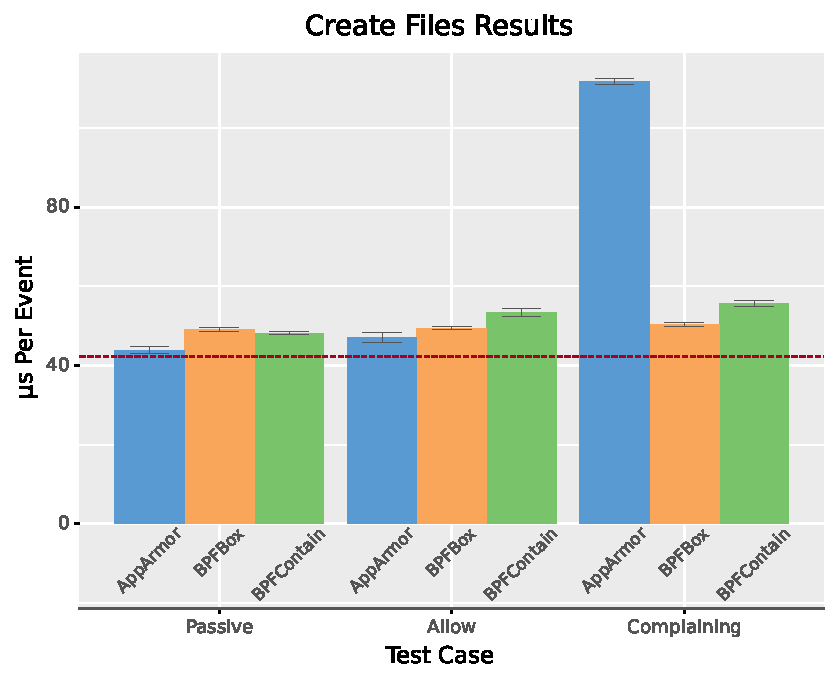
\includegraphics[width=0.45\linewidth]{results/graphs/Create-Files.pdf}%
  }\qquad
  \subfloat{
    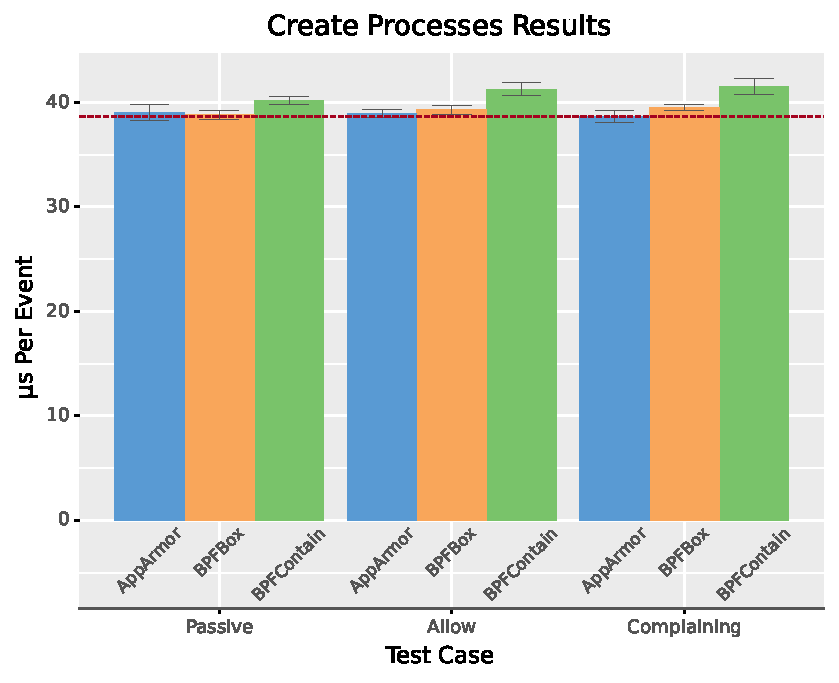
\includegraphics[width=0.45\linewidth]{results/graphs/Create-Processes.pdf}%
  }\\
  \subfloat{
    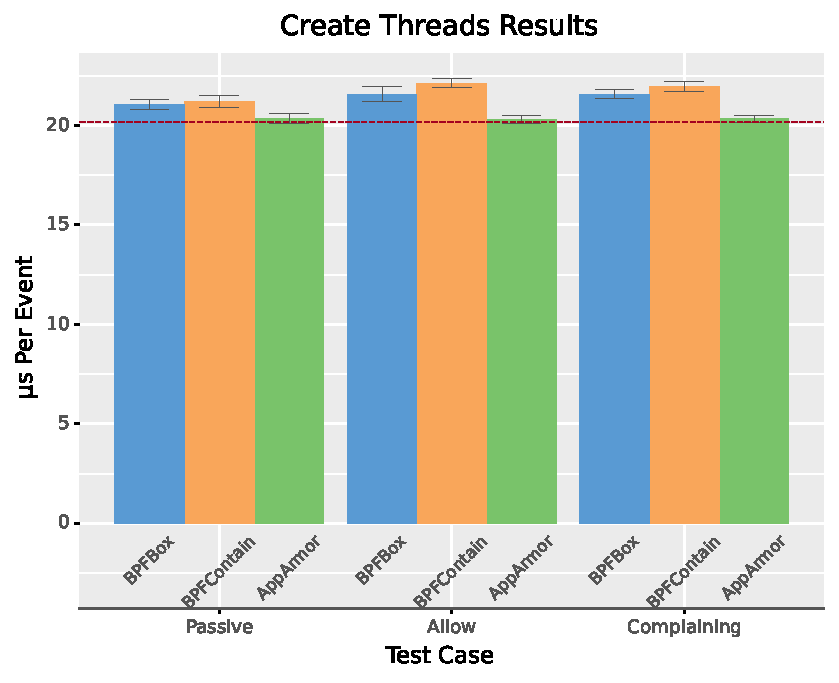
\includegraphics[width=0.45\linewidth]{results/graphs/Create-Threads.pdf}%
  }\qquad
  \subfloat{
    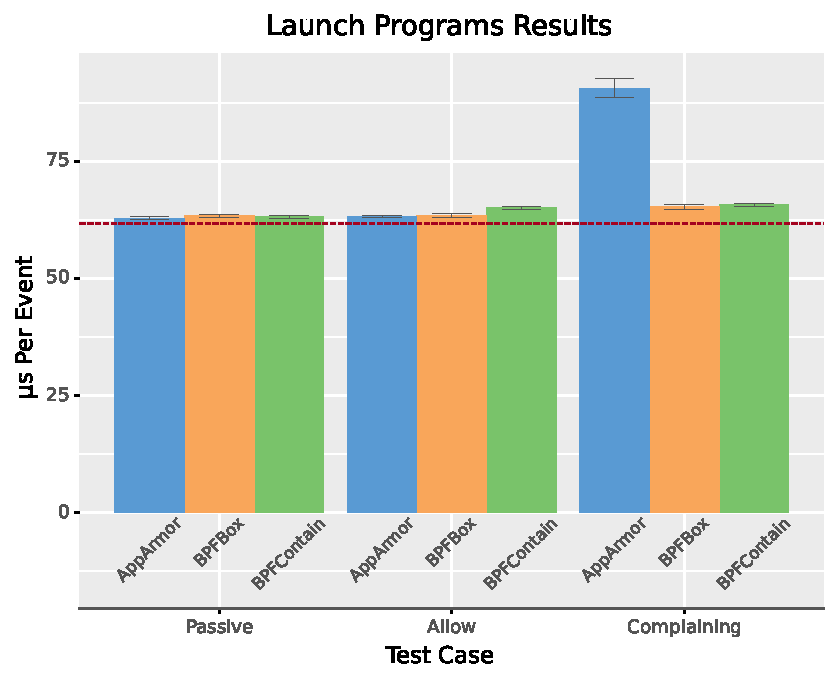
\includegraphics[width=0.45\linewidth]{results/graphs/Launch-Programs.pdf}%
  }\\
  \subfloat{
    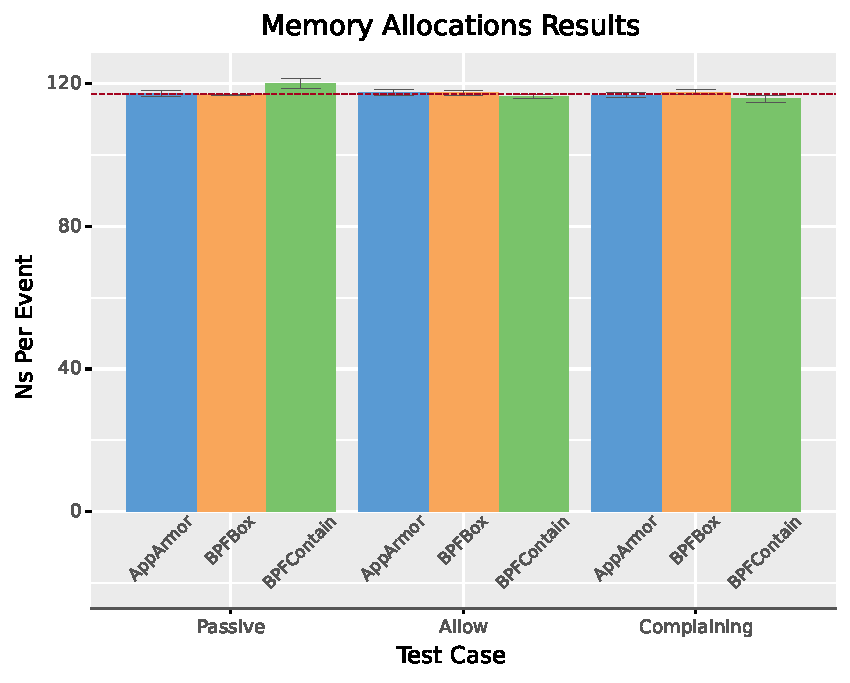
\includegraphics[width=0.45\linewidth]{results/graphs/Memory-Allocations.pdf}%
  }
  \caption[The results of the OSBench micro-benchmarks]{
    The results of the OSBench micro-benchmarks. The error bars show standard
    deviation and the red lines show base measurements for each test. Lower times are
    better.
  }%
  \label{fig:osbench}
\end{figure}

\subsubsection{OSBench File Creation}

The file creation benchmark (\Cref{tab:phoronix-create-files} and \Cref{fig:osbench}) indicates
that \bpfbox{} and \bpfcontain{} have significantly higher overhead than AppArmor in the
\textbf{Passive} and \textbf{Allow} cases. \bpfcontain{}, in particular, performs the worst
out of the three systems in these two cases. This poor performance can be
explained by the fact that it is an unoptimized research prototype, and that it performs
complex analysis on filesystem operations to come to a policy decision. Conversely,
AppArmor is a well-established security mechanism which has undergone significant
performance optimizations over time. Future optimizations on \bpfcontain{} can
significantly improve its performance overhead in practice. Despite a seemingly high
performance overhead in the \textbf{Passive} and \textbf{Allow} cases, \bpfbox{} and
\bpfcontain{} incur a performance penalty of under 12$\mu$s each, a slowdown which should
be acceptable in practice.  Moreover, in the \textbf{Complain} case, \bpfbox{} and
\bpfcontain{} significantly outperform AppArmor. This result can be attributed to
implementation differences in their event-logging mechanisms.

\begin{table}[htp!]
\centering
\footnotesize
\caption[Results of the create files benchmark]{Results of the create files benchmark. Units are $\mu$s Per Event. Lower is better. Percent overhead is compared to the baseline result.}
\label{tab:phoronix-create-files}
\begin{tabular}{llrrr}
\toprule
            &          &    Mean &   Std &  Overhead \\
Test Case & System &         &       &           \\
\midrule
Base & --- &   42.21 &  1.22 &       --- \\
\cline{1-5}
\multirow{3}{*}{Passive} & BPFBox &   49.09 &  0.40 &   16.31\% \\
            & BPFContain &   48.16 &  0.36 &   14.11\% \\
            & AppArmor &   43.87 &  0.95 &    3.93\% \\
\cline{1-5}
\multirow{3}{*}{Allow} & BPFBox &   49.41 &  0.39 &   17.08\% \\
            & BPFContain &   53.43 &  1.01 &   26.60\% \\
            & AppArmor &   47.07 &  1.15 &   11.52\% \\
\cline{1-5}
\multirow{3}{*}{Complaining} & BPFBox &   50.34 &  0.54 &   19.27\% \\
            & BPFContain &   55.67 &  0.75 &   31.89\% \\
            & AppArmor &  111.66 &  0.75 &  164.55\% \\
\bottomrule
\end{tabular}
\end{table}

% \begingroup\small
% \begin{longtable}[c]{llrrr}
%   \caption[Results of the file creation benchmark]{
%     Results of the file creation benchmark. Units are $\mu$s per event; lower is
%     better. Percent overhead is compared to the baseline result.
%   }%
%   \label{tab:phoronix-files}\\
%   \toprule
%    Test Case & System         &  Mean  & Std & Overhead (\%)\\
%    \midrule
%    Base      & ---            &  42.21 & 1.22 &  ---     \\
%    \midrule
%    Passive   & \bpfbox{}      &  49.09 & 0.40 &  16.31\% \\
%              & \bpfcontain{}  &  48.16 & 0.36 &  14.11\% \\
%              & AppArmor       &  43.87 & 0.95 &   3.93\% \\
%    \midrule
%    Allow     & \bpfbox{}      &  49.41 & 0.39 &  17.08\% \\
%              & \bpfcontain{}  &  53.43 & 1.01 &  26.60\% \\
%              & AppArmor       &  47.07 & 1.15 &  11.52\% \\
%    \midrule
%    Complain  & \bpfbox{}      &  50.34 & 0.54 &  19.27\% \\
%              & \bpfcontain{}  &  55.67 & 0.75 &  31.89\% \\
%              & AppArmor       & 111.66 & 0.75 & 164.55\% \\
%   \bottomrule
% \end{longtable}
% \endgroup

In the \textbf{Passive} case, \bpfbox{} and \bpfcontain{}'s high performance overhead can
be attributed to the fact that they each invoke multiple \gls{bpf} programs over multiple
\gls{lsm} hooks on the \texttt{open(2)}, \texttt{write(2)}, and \texttt{unlink(2)} code
paths. Unlike AppArmor, \bpfbox{} and \bpfcontain{} invoke a new \gls{ebpf} program on
every \gls{lsm} hook along this code path, then perform a map lookup to determine whether
the process is being actively traced. The overhead associated with this many \gls{bpf}
program invocations is non-trivial compared with the overhead of simply calling into an
\gls{lsm} hook. Future improvements to the \gls{krsi} framework may also be able to reduce
the performance overhead of \gls{bpf} \gls{lsm} programs.

In the \textbf{Allow} case, \bpfbox{} is more in line with AppArmor, while \bpfcontain{}
is shown to exhibit a slightly higher overhead. However, as with the \textbf{Passive}
case, this overhead should be acceptable in practice. We can attribute the additional
overhead shown by \bpfcontain{} to the nuances associated with its code path for file and
filesystem policies. For each file operation, \bpfcontain{} performs multiple map queries
and reads information from multiple kernel data structures to enforce its default policy.
Future iterations of \bpfcontain{} may improve this overhead by caching policy decisions
for filesystem objects and/or resolving inefficiencies in how \bpfcontain{} reads
information from kernel data structures.

In the \textbf{Complaining} case, \bpfbox{} and \bpfcontain{} significantly outperform
AppArmor, a fact which can be attributed to inefficiencies in AppArmor's logging
mechanism, which relies on the kernel's audit framework. The ring buffer maps used by
\bpfbox{} and \bpfcontain{} are known to exhibit comparatively less
overhead~\cite{zeng2015_auditing, zhang2021_lsm_file_overhead, nakryiko2020_ringbuf}.
Additional overhead may also arise due to differences in how AppArmor translates files and
access patterns to log messages.

\subsubsection{OSBench Process Creation}

The results of the process creation benchmark (\Cref{tab:phoronix-create-processes} and \Cref{fig:osbench}) indicate
that \bpfbox{} and \bpfcontain{} introduce modest overhead on top of the \texttt{fork(2)}
system call.  Comparatively, AppArmor introduces very little overhead, well within the
margin of error for measurements. The additional overhead introduced by \bpfbox{} and
\bpfcontain{} can be explained by the additional per-process and per-thread accounting
performed by each system. \bpfcontain{}, in particular, handles a significant amount of
per-process and per-thread metadata, which must be populated each time a \texttt{fork(2)}
or \texttt{clone(2)} occurs, and cleaned up each time a process exits. However, it should
be noted that both \bpfbox{} and \bpfcontain{} introduce less than $10\%$ overhead along
this code path (within 1--2$\mu$s), which should be imperceptible in practice.

% \begin{figure}[htp]
%   \centering
%   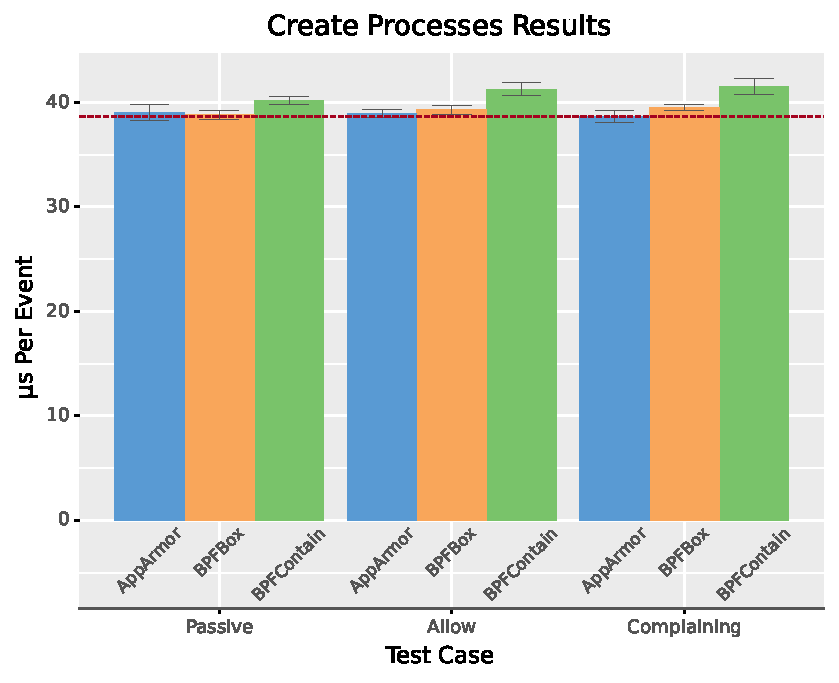
\includegraphics[width=0.8\linewidth]{results/graphs/Create-Processes.pdf}
%   \caption{
%     Results of the process creation benchmark.
%     The error bars show standard deviation and the red line shows the base measurement.
%     Lower times are better.
%   }%
%   \label{fig:phoronix-processes}
% \end{figure}

\begin{table}[htp!]
\centering
\footnotesize
\caption[Results of the create processes benchmark]{Results of the create processes benchmark. Units are $\mu$s Per Event. Lower is better. Percent overhead is compared to the baseline result.}
\label{tab:phoronix-create-processes}
\begin{tabular}{llrrr}
\toprule
            &          &   Mean &   Std & Overhead \\
Test Case & System &        &       &          \\
\midrule
Base & --- &  38.65 &  0.36 &      --- \\
\cline{1-5}
\multirow{3}{*}{Passive} & BPFBox &  38.81 &  0.44 &   0.40\% \\
            & BPFContain &  40.17 &  0.39 &   3.93\% \\
            & AppArmor &  39.04 &  0.74 &   1.01\% \\
\cline{1-5}
\multirow{3}{*}{Allow} & BPFBox &  39.28 &  0.41 &   1.63\% \\
            & BPFContain &  41.27 &  0.63 &   6.77\% \\
            & AppArmor &  38.94 &  0.34 &   0.74\% \\
\cline{1-5}
\multirow{3}{*}{Complaining} & BPFBox &  39.51 &  0.33 &   2.22\% \\
            & BPFContain &  41.49 &  0.76 &   7.33\% \\
            & AppArmor &  38.68 &  0.56 &   0.07\% \\
\bottomrule
\end{tabular}
\end{table}

% \begingroup\small
% \begin{longtable}[c]{llrrr}
%   \caption[Results of the process creation benchmark]{
%     Results of the process creation benchmark. Units are $\mu$s per event; lower is
%     better. Percent overhead is compared to the baseline result.
%   }%
%   \label{tab:phoronix-processes}\\
%   \toprule
%    Test Case & System         &  Mean & Std & Overhead (\%)\\
%    \midrule
%    Base      & ---            & 38.65 & 0.36 &  ---    \\
%    \midrule
%    Passive   & \bpfbox{}      & 38.81 & 0.44 &  0.40\% \\
%              & \bpfcontain{}  & 40.17 & 0.39 &  3.93\% \\
%              & AppArmor       & 39.04 & 0.74 &  1.01\% \\
%    \midrule
%    Allow     & \bpfbox{}      & 39.28 & 0.41 &  1.63\% \\
%              & \bpfcontain{}  & 41.27 & 0.63 &  6.77\% \\
%              & AppArmor       & 38.94 & 0.34 &  0.74\% \\
%    \midrule
%    Complain  & \bpfbox{}      & 39.51 & 0.33 &  2.22\% \\
%              & \bpfcontain{}  & 41.49 & 0.76 &  7.33\% \\
%              & AppArmor       & 38.68 & 0.56 &  0.07\% \\
%   \bottomrule
% \end{longtable}
% \endgroup

\subsubsection{OSBench Thread Creation}

The thread creation results (\Cref{tab:phoronix-create-threads} and \Cref{fig:osbench}) are directly related to the
process creation results discussed above, insofar as both operations exercise the same
\gls{bpf} programs in \bpfbox{} and \bpfcontain{}. Since thread creation is faster then
process creation, the percentage overhead of \bpfbox{} and \bpfcontain{} appear
comparatively higher, but the underlying delta is the same, at roughly 1--2$\mu$s per
event. Despite these differences in thread and process creation speeds, the resulting
percentage overhead of \bpfbox{} and \bpfcontain{} is still under 10\%.

% \begin{figure}[htp]
%   \centering
%   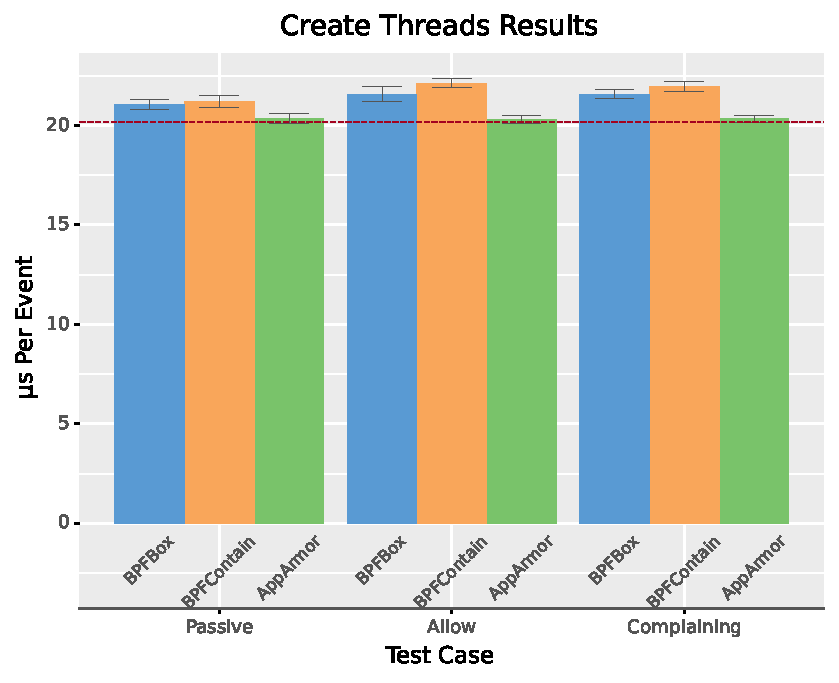
\includegraphics[width=0.8\linewidth]{results/graphs/Create-Threads.pdf}
%   \caption{
%     Results of the thread creation benchmark.
%     The error bars show standard deviation and the red line shows the base measurement.
%     Lower times are better.
%   }%
%   \label{fig:phoronix-threadsa}
% \end{figure}

\begin{table}[ht!]
\centering
\footnotesize
\caption[Results of the Create Threads benchmark]{Results of the Create Threads benchmark. Units are $\mu$s per event. Lower is better. Percent overhead is compared to the baseline result.}
\label{tab:phoronix-create-threads}
\begin{tabular}{llrrr}
\toprule
            &          &   Mean &   Std & Overhead \\
Test Case & System &        &       &          \\
\midrule
Base & --- &  20.18 &  0.19 &      --- \\
\cline{1-5}
\multirow{3}{*}{Passive} & BPFBox &  21.06 &  0.25 &   4.37\% \\
            & BPFContain &  21.21 &  0.30 &   5.08\% \\
            & AppArmor &  20.32 &  0.25 &   0.71\% \\
\cline{1-5}
\multirow{3}{*}{Allow} & BPFBox &  21.56 &  0.37 &   6.84\% \\
            & BPFContain &  22.11 &  0.22 &   9.53\% \\
            & AppArmor &  20.29 &  0.18 &   0.54\% \\
\cline{1-5}
\multirow{3}{*}{Complaining} & BPFBox &  21.57 &  0.25 &   6.90\% \\
            & BPFContain &  21.96 &  0.24 &   8.80\% \\
            & AppArmor &  20.32 &  0.16 &   0.70\% \\
\bottomrule
\end{tabular}
\end{table}

% \begingroup\small
% \begin{longtable}[c]{llrrr}
%   \caption[Results of the thread creation benchmark]{
%     Results of the thread creation benchmark. Units are $\mu$s per event; lower is
%     better. Percent overhead is compared to the baseline result.
%   }%
%   \label{tab:phoronix-threads}\\
%   \toprule
%    Test Case & System         &  Mean & Std  & Overhead (\%)\\
%    \midrule
%    Base      & ---            & 20.18 & 0.19 & ---     \\
%    \midrule
%    Passive   & \bpfbox{}      & 21.06 & 0.25 & 4.37\% \\
%              & \bpfcontain{}  & 21.21 & 0.30 & 5.08\% \\
%              & AppArmor       & 20.32 & 0.25 & 0.71\% \\
%    \midrule
%    Allow     & \bpfbox{}      & 21.56 & 0.37 & 6.84\% \\
%              & \bpfcontain{}  & 22.11 & 0.22 & 9.53\% \\
%              & AppArmor       & 20.29 & 0.18 & 0.54\% \\
%    \midrule
%    Complain  & \bpfbox{}      & 21.57 & 0.25 & 6.90\% \\
%              & \bpfcontain{}  & 21.96 & 0.24 & 8.80\% \\
%              & AppArmor       & 20.32 & 0.16 & 0.70\% \\
%   \bottomrule
% \end{longtable}
% \endgroup

\subsubsection{OSBench Program Launching}

The launch programs benchmark (\Cref{tab:phoronix-launch-programs} and \Cref{fig:osbench}) is essentially the
same as the process creation benchmark (c.f.~\Cref{tab:phoronix-create-processes}), with one
major difference: the addition of an \texttt{execve(2)} call after the \texttt{clone(2)}
system call. This \texttt{execve(2)} call adds a constant overhead of about 20$\mu$s on
top of the original process creation results, as well as additional \gls{lsm} hook
invocations along the \texttt{execve(2)} code path. These factors contribute to \bpfbox{}
and \bpfcontain{} performing slightly worse than AppArmor in the \textbf{Passive} and
\textbf{Allow} cases and significantly better than AppArmor in the \textbf{Complaining}
case.

The additional \gls{lsm} hook invocations caused by the \texttt{execve(2)} severely impact
AppArmor's performance in the \textbf{Complaining} case, for the same reasons as discussed
in the file creation results (c.f.~\Cref{tab:phoronix-create-files}). \bpfbox{} and \bpfcontain{}
exhibit comparatively little overhead, despite the \texttt{execve(2)} call. This result
can be explained by the fact that \texttt{execve(2)}'s code path invokes significantly
fewer \gls{lsm} hooks than the file creation and deletion code paths we examined earlier.
In all test cases, \bpfbox{} and \bpfcontain{} are able to achieve under $7\%$ overhead in
the worst case, and under $3\%$ in the majority of cases.

% \begin{figure}[htp]
%   \centering
%   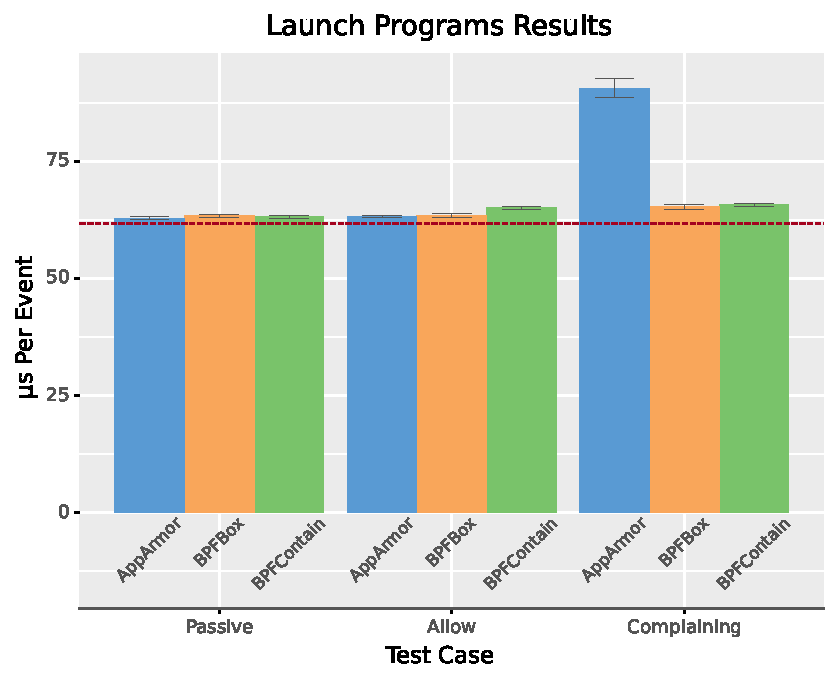
\includegraphics[width=0.8\linewidth]{results/graphs/Launch-Programs.pdf}
%   \caption{
%     Results of the program launching benchmark.
%     The error bars show standard deviation and the red line shows the base measurement.
%     Lower times are better.
%   }%
%   \label{fig:phoronix-launch-programs}
% \end{figure}

\begin{table}[htp!]
\centering
\footnotesize
\caption[Results of the launch programs benchmark]{Results of the launch programs benchmark. Units are $\mu$s Per Event. Lower is better. Percent overhead is compared to the baseline result.}
\label{tab:phoronix-launch-programs}
\begin{tabular}{llrrr}
\toprule
            &          &   Mean &   Std & Overhead \\
Test Case & System &        &       &          \\
\midrule
Base & --- &  61.67 &  0.20 &      --- \\
\cline{1-5}
\multirow{3}{*}{Passive} & BPFBox &  63.30 &  0.28 &   2.64\% \\
            & BPFContain &  63.12 &  0.28 &   2.34\% \\
            & AppArmor &  62.84 &  0.25 &   1.89\% \\
\cline{1-5}
\multirow{3}{*}{Allow} & BPFBox &  63.44 &  0.40 &   2.86\% \\
            & BPFContain &  65.05 &  0.38 &   5.47\% \\
            & AppArmor &  63.17 &  0.21 &   2.43\% \\
\cline{1-5}
\multirow{3}{*}{Complaining} & BPFBox &  65.22 &  0.48 &   5.75\% \\
            & BPFContain &  65.66 &  0.30 &   6.47\% \\
            & AppArmor &  90.56 &  1.97 &  46.83\% \\
\bottomrule
\end{tabular}
\end{table}

% \begingroup\small
% \begin{longtable}[c]{llrrr}
%   \caption[Results of the program launching benchmark]{
%     Results of the program launching benchmark. Units are $\mu$s per event; lower is
%     better. Percent overhead is compared to the baseline result.
%   }%
%   \label{tab:phoronix-launch-programs}\\
%   \toprule
%    Test Case & System         &  Mean & Std  & Overhead (\%)\\
%    \midrule
%    Base      & ---            & 61.67 & 0.20 & ---     \\
%    \midrule
%    Passive   & \bpfbox{}      & 63.30 & 0.28 & 2.64 \% \\
%              & \bpfcontain{}  & 63.12 & 0.28 & 2.34 \% \\
%              & AppArmor       & 62.84 & 0.25 & 1.89 \% \\
%    \midrule
%    Allow     & \bpfbox{}      & 63.44 & 0.40 & 2.86 \% \\
%              & \bpfcontain{}  & 65.05 & 0.38 & 5.47 \% \\
%              & AppArmor       & 63.17 & 0.21 & 2.43 \% \\
%    \midrule
%    Complain  & \bpfbox{}      & 65.22 & 0.48 & 5.75 \% \\
%              & \bpfcontain{}  & 65.66 & 0.30 & 6.47 \% \\
%              & AppArmor       & 90.56 & 1.97 & 46.83\% \\
%   \bottomrule
% \end{longtable}
% \endgroup

\subsubsection{OSBench Memory Allocations}

The memory allocation benchmark (\Cref{tab:phoronix-memory-allocations} and
\Cref{fig:osbench}) indicates that none of the systems had any significant affect on
memory allocation. In some cases, percent overhead falsely appears to indicate
a performance \textit{improvement}, which we attribute to measurement error rather than
any indication of increased performance. This result is consistent with expectations,
since memory allocation does not directly interact with any \gls{lsm} hooks in the kernel,
and neither \bpfbox{} nor \bpfcontain{} instruments any \gls{bpf} programs on the heap
allocation code path.

\begin{table}[ht!]
\centering
\footnotesize
\caption[Results of the Memory Allocations benchmark]{Results of the Memory Allocations benchmark. Units are ns per event. Lower is better. Percent overhead is compared to the baseline result.}
\label{tab:phoronix-memory-allocations}
\begin{tabular}{llrrr}
\toprule
            &          &    Mean &   Std & Overhead \\
Test Case & System &         &       &          \\
\midrule
Base & --- &  117.17 &  0.67 &      --- \\
\cline{1-5}
\multirow{3}{*}{Passive} & BPFBox &  116.87 &  0.18 &  -0.26\% \\
            & BPFContain &  120.05 &  1.27 &   2.46\% \\
            & AppArmor &  117.24 &  0.97 &   0.06\% \\
\cline{1-5}
\multirow{3}{*}{Allow} & BPFBox &  117.41 &  0.71 &   0.21\% \\
            & BPFContain &  116.42 &  0.62 &  -0.64\% \\
            & AppArmor &  117.49 &  0.81 &   0.28\% \\
\cline{1-5}
\multirow{3}{*}{Complaining} & BPFBox &  117.62 &  0.75 &   0.38\% \\
            & BPFContain &  115.73 &  1.04 &  -1.22\% \\
            & AppArmor &  116.81 &  0.80 &  -0.31\% \\
\bottomrule
\end{tabular}
\end{table}


% \begin{figure}[htp]
%   \centering
%   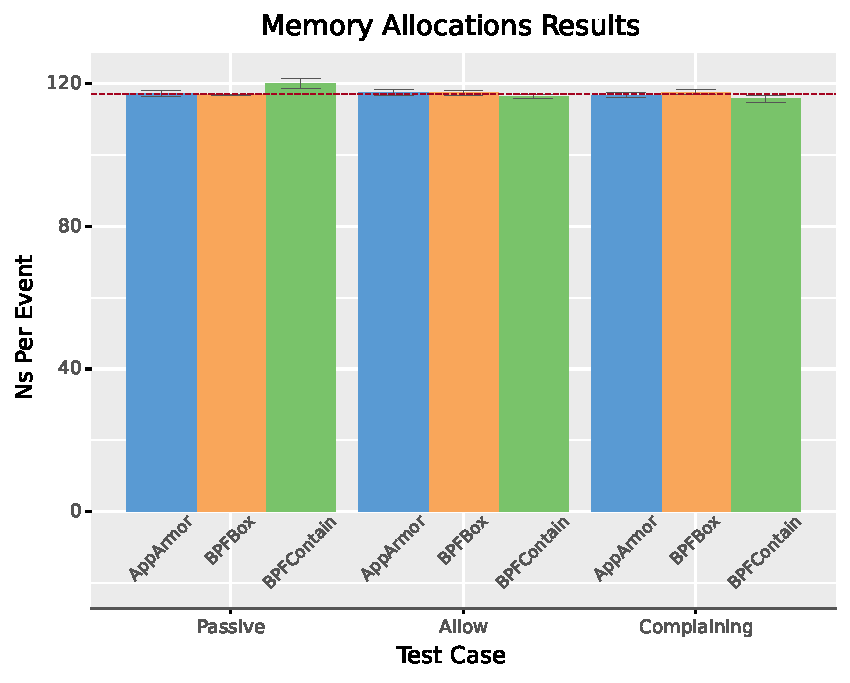
\includegraphics[width=0.8\linewidth]{results/graphs/Memory-Allocations.pdf}
%   \caption{
%     Results of the memory allocation benchmark.
%     The error bars show standard deviation and the red line shows the base measurement.
%     Lower times are better.
%   }%
%   \label{fig:phoronix-memory}
% \end{figure}
% \begingroup\small
% \begin{longtable}[c]{llrrr}
%   \caption[Results of the memory allocation benchmark]{
%     Results of the memory allocation benchmark. Units are Ns per event; lower is
%     better. Percent overhead is compared to the baseline result.
%   }%
%   \label{tab:phoronix-memory}\\
%   \toprule
%    Test Case & System         &  Mean  & Std  & Overhead (\%)\\
%    \midrule
%    Base      & ---            & 117.17 & 0.67 & ---     \\
%    \midrule
%    Passive   & \bpfbox{}      & 116.87 & 0.18 & -0.26\% \\
%              & \bpfcontain{}  & 120.05 & 1.27 &  2.46\% \\
%              & AppArmor       & 117.24 & 0.97 &  0.06\% \\
%    \midrule
%    Allow     & \bpfbox{}      & 117.41 & 0.71 &  0.21\% \\
%              & \bpfcontain{}  & 116.42 & 0.62 & -0.64\% \\
%              & AppArmor       & 117.49 & 0.81 &  0.28\% \\
%    \midrule
%    Complain  & \bpfbox{}      & 117.62 & 0.75 &  0.38\% \\
%              & \bpfcontain{}  & 115.73 & 1.04 & -1.22\% \\
%              & AppArmor       & 116.81 & 0.80 & -0.31\% \\
%   \bottomrule
% \end{longtable}
% \endgroup


\subsubsection{Kernel Compilation Results}

The kernel compilation benchmark (\Cref{tab:phoronix-kernel-compilation} and
\Cref{fig:phoronix-kernel}) provides a representative depiction of overhead for
a computationally-heavy task that involves multiple processes and significant amounts of
file I/O. The results of this benchmark indicate that \bpfbox{} and \bpfcontain{} exhibit
performance overhead that is roughly consistent with AppArmor in the average case. The
\textbf{Passive} and \textbf{Allow} results indicate that all three systems exhibit an
acceptable performance overhead of under about $3\%$. The \textbf{Complain} results
indicate that \bpfcontain{} performs significantly better than both \bpfbox{} and AppArmor
under a large event logging volume. This result can be attributed to minor implementation
details, including improvements in how \bpfcontain{} handles event logging from multiple
distinct sources.
%This result can likely be
%attributed to \bpfcontain{}'s more efficient userspace implementation in Rust, which
%significantly outperforms the \bpfbox{} Python implementation.

\begin{table}[htp!]
\centering
\footnotesize
\caption[Results of the kernel compilation benchmark]{Results of the kernel compilation benchmark. Units are Seconds. Lower is better. Percent overhead is compared to the baseline result.}
\label{tab:phoronix-kernel-compilation}
\begin{tabular}{llrrr}
\toprule
            &          &    Mean &   Std & Overhead \\
Test Case & System &         &       &          \\
\midrule
Base & --- &  235.32 &  1.96 &      --- \\
\cline{1-5}
\multirow{3}{*}{Passive} & BPFBox &  237.95 &  1.88 &   1.12\% \\
            & BPFContain &  237.63 &  2.08 &   0.98\% \\
            & AppArmor &  236.45 &  1.92 &   0.48\% \\
\cline{1-5}
\multirow{3}{*}{Allow} & BPFBox &  238.23 &  2.19 &   1.24\% \\
            & BPFContain &  243.09 &  2.19 &   3.30\% \\
            & AppArmor &  237.59 &  2.04 &   0.97\% \\
\cline{1-5}
\multirow{3}{*}{Complaining} & BPFBox &  269.64 &  1.98 &  14.59\% \\
            & BPFContain &  244.80 &  2.04 &   4.03\% \\
            & AppArmor &  288.54 &  2.11 &  22.62\% \\
\bottomrule
\end{tabular}
\end{table}


\begin{table}[ht!]
\centering
\footnotesize
\caption[Results of the Apache benchmark]{Results of the Apache benchmark. Units are requests per second. Higher is better. Percent overhead is compared to the baseline result.}
\label{tab:phoronix-apache}
\begin{tabular}{llrrr}
\toprule
            &          &      Mean &     Std & Overhead \\
Test Case & System &           &         &          \\
\midrule
Base & --- &  20576.49 &  281.94 &      --- \\
\cline{1-5}
\multirow{3}{*}{Passive} & BPFBox &  19946.04 &  233.62 &   3.06\% \\
            & BPFContain &  19530.92 &  317.95 &   5.08\% \\
            & AppArmor &  20363.42 &  331.64 &   1.04\% \\
\cline{1-5}
\multirow{3}{*}{Allow} & BPFBox &  19465.86 &  253.81 &   5.40\% \\
            & BPFContain &  18934.55 &  299.23 &   7.98\% \\
            & AppArmor &  20276.95 &   64.30 &   1.46\% \\
\cline{1-5}
\multirow{3}{*}{Complaining} & BPFBox &  20139.10 &  101.59 &   2.13\% \\
            & BPFContain &  18293.09 &  160.00 &  11.10\% \\
            & AppArmor &  19827.05 &  298.27 &   3.64\% \\
\bottomrule
\end{tabular}
\end{table}

% \begingroup\small
% \begin{longtable}[c]{llrrr}
%   \caption[Results of the kernel compilation benchmark]{
%     Results of the kernel compilation benchmark. Units are seconds to compile; lower is
%     better. Percent overhead is compared to the baseline result.
%   }%
%   \label{tab:phoronix-kernel}\\
%   \toprule
%    Test Case & System         &  Mean  & Std  & Overhead (\%)\\
%    \midrule
%    Base      & ---            & 235.32 & 1.96 & ---     \\
%    \midrule
%    Passive   & \bpfbox{}      & 237.95 & 1.88 &  1.12\% \\
%              & \bpfcontain{}  & 237.63 & 2.08 &  0.98\% \\
%              & AppArmor       & 236.45 & 1.92 &  0.48\% \\
%    \midrule
%    Allow     & \bpfbox{}      & 238.23 & 2.19 &  1.24\% \\
%              & \bpfcontain{}  & 243.09 & 2.19 &  3.30\% \\
%              & AppArmor       & 237.59 & 2.04 &  0.97\% \\
%    \midrule
%    Complain  & \bpfbox{}      & 269.64 & 1.98 & 14.59\% \\
%              & \bpfcontain{}  & 244.81 & 2.04 &  4.03\% \\
%              & AppArmor       & 288.54 & 2.11 & 22.62\% \\
%   \bottomrule
% \end{longtable}
% \endgroup

\begin{figure}[htp]
  \centering
  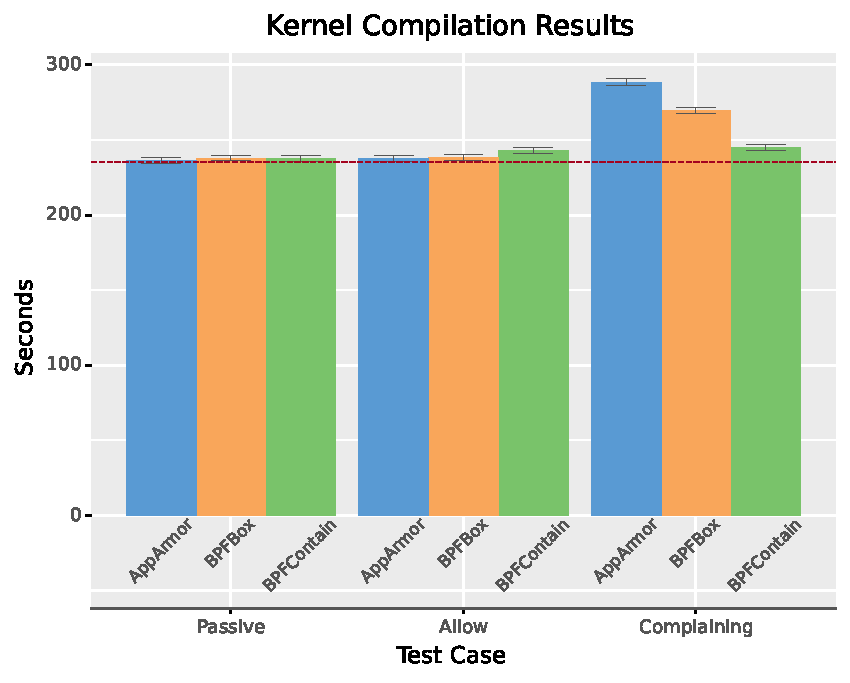
\includegraphics[width=0.6\linewidth]{results/graphs/Kernel-Compilation.pdf}
  \caption[Results of the kernel compilation benchmark]{
    Results of the kernel compilation benchmark.
    The error bars show standard deviation and the red line shows the base measurement.
    Lower times are better.
  }%
  \label{fig:phoronix-kernel}
\end{figure}

\begin{figure}[htp]
  \centering
  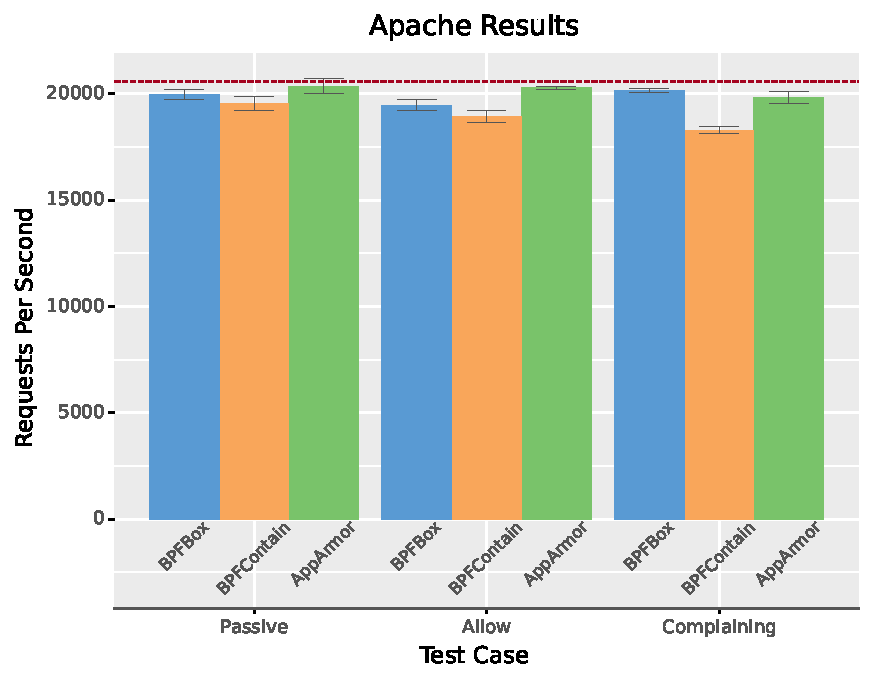
\includegraphics[width=0.6\linewidth]{results/graphs/Apache.pdf}
  \caption[Results of the Apache web server benchmark]{
    Results of the Apache web server benchmark.
    The error bars show standard deviation and the red line shows the base measurement.
    Higher requests per second are better.
  }%
  \label{fig:phoronix-apache}
\end{figure}


\subsubsection{Apache Web Server Results}

The Apache web server benchmark (\Cref{tab:phoronix-apache} and \Cref{fig:phoronix-apache}) indicates that, while
\bpfbox{} and \bpfcontain{} do exhibit a higher performance overhead than AppArmor, this
overhead is still within an acceptable range at around $11\%$ in the worst case for
\bpfcontain{}. This overhead should still be quite acceptable in practice, and can be
improved through further optimizations in \bpfcontain{}'s enforcement engine, which is
still in the prototype phase. The results from the \textbf{Complain} case appear to
indicate a slight performance improvement for \bpfbox{} over AppArmor; this is likely due
to variance in the measurements rather than a true performance improvement, as the
difference between the two systems falls within the margin of error.

% \begingroup\small
% \begin{longtable}[c]{llrrr}
%   \caption[Results of the Apache web server benchmark]{
%     Results of the Apache web server benchmark. Units are requests per second; higher is
%     better. Percent overhead is compared to the baseline result.
%   }%
%   \label{tab:phoronix-apache}\\
%   \toprule
%    Test Case & System         &  Mean   & Std   & Overhead (\%)\\
%    \midrule
%    Base      & ---            & 20576.49 & 281.94 & ---     \\
%    \midrule
%    Passive   & \bpfbox{}      & 19946.04 & 233.62 &  3.06\% \\
%              & \bpfcontain{}  & 19530.92 & 317.95 &  5.08\% \\
%              & AppArmor       & 20363.42 & 331.64 &  1.04\% \\
%    \midrule
%    Allow     & \bpfbox{}      & 19465.86 & 253.81 &  5.40\% \\
%              & \bpfcontain{}  & 18934.55 & 299.23 &  7.98\% \\
%              & AppArmor       & 20276.95 &  64.30 &  1.46\% \\
%    \midrule
%    Complain  & \bpfbox{}      & 20139.10 & 101.59 &  2.13\% \\
%              & \bpfcontain{}  & 18293.09 & 160.00 & 11.10\% \\
%              & AppArmor       & 19827.05 & 298.27 &  3.64\% \\
%   \bottomrule
% \end{longtable}
% \endgroup

% \subsubsection{\glsentryshort{ipc} Results}

\subsection{Discussion of Results}%
\label{ss:eval-performance-discussion}

The results of the benchmarking tests show that both \bpfbox{} and \bpfcontain{} incur
acceptable performance overhead in practice. In many cases, overhead is competitive with
AppArmor, a standard \gls{lsm} that ships with the stock Linux kernel. In other cases, the
performance overhead of \bpfbox{} and \bpfcontain{} is higher than that of AppArmor, but
still within an acceptable range, such that the slowdown should be either imperceptible or
acceptable in most practical use cases.  As \bpfbox{} and \bpfcontain{} are both research
prototypes, they have not yet been optimized to the extent that AppArmor has. This lack of
optimization is particularly evident in the results for \bpfcontain{}, and may account for
significant differences in performance in the file I/O and Apache web server tests.

\begin{table}[ht]
  \centering
  \footnotesize
  \caption[Geometric means of Phoronix benchmarking results]{
    Geometric means of Phoronix benchmarking results, as provided by the Phoronix Test
    Suite. These are indicative of overall performance across all tests. For test case,
    percent change from the base results are also given. Higher values are better.
  }%
  \label{tab:phoronix-geometric}
  \begin{tabular}{llrr}
  \toprule
             &               & Geom. Mean & Overhead (\%)\\
   Test Case & System        &            &              \\
   \midrule
   Base      &               & 6.238          & --- \\
   \cline{1-4}
   Passive   & \bpfbox{}     & 6.007          & 3.70\% \\
             & \bpfcontain{} & 5.951          & 4.60\% \\
             & AppArmor      & 6.158          & 1.28\% \\
   \cline{1-4}
   Allow     & \bpfbox{}     & 5.944          & 4.71\% \\
             & \bpfcontain{} & 5.763          & 7.61\% \\
             & AppArmor      & 6.086          & 2.35\% \\
   \cline{1-4}
   Complain  & \bpfbox{}     & 5.823          & 6.65\% \\
             & \bpfcontain{} & 5.693          & 8.74\% \\
             & AppArmor      & 4.962          & 20.46\% \\
  \bottomrule
  \end{tabular}
\end{table}

While \bpfbox{} and \bpfcontain{} are not as efficient as AppArmor in the \textbf{Passive}
and \textbf{Allow}  test cases, the additional performance overhead should be an
acceptable price to pay for the increase in flexibility and system observability afforded
by an \gls{ebpf} implementation as opposed to a traditional Linux Security Module.
Moreover, \bpfcontain{} extends \bpfbox{}'s original enforcement model, adding new rule categories
and enforcement defaults. While these enhancements may be the cause of some additional
performance overhead, we attribute the majority of \bpfcontain{}'s actual performance
overhead to sub-optimal memory allocations and data structure access patterns, which can
be optimized in the future.

Despite under-performing in the \textbf{Passive} and \textbf{Allow} cases, both \bpfbox{}
and \bpfcontain{} significantly outperform AppArmor in the \textbf{Complain} test case,
due to a more efficient event logging mechanism.  \Cref{tab:phoronix-geometric} shows the
geometric mean of all tests for each test case, indicating that \bpfbox{} and
\bpfcontain{} exhibit and average performance penalty of under $9\%$ in practice, while
AppArmor can exhibit overheads of up to $20\%$ in the worst case.

Although the results presented in this section indicate a comparative performance with
AppArmor, many other widely-adopted \glspl{lsm} can perform significantly worse than
AppArmor in some cases. For instance, Zhang \etal~\cite{zhang2021_lsm_file_overhead} found
that SELinux, perhaps the most widely-used Linux \gls{mac} implementation, exhibits
significant performance overhead, many times worse than AppArmor in some cases. These
results could indicate that \bpfbox{} and \bpfcontain{} might perform favourably compared
to alternative \glspl{lsm} like SELinux, although further investigation is needed in order
to establish a direct comparison.

\section{Security Analysis}%
\label{s:eval-security}

We now turn our attention to the security of \bpfbox{} and \bpfcontain. Specifically, we
conduct an informal security analysis on both systems, evaluating how well they are able
to confine an attacker under the threat model presented in \Cref{s:cp-threat-model} of
\Cref{c:confinement-problem}. In particular, we examine the various policy rule categories
provided by both \bpfbox{} and \bpfcontain{} as well as how their respective enforcement
engines enforce policy at runtime. We characterize an adversary's ability to escape
confinement based on whether the adversary is able to violate the security assumptions of
\bpfbox{} and \bpfcontain{} under a policy designed to prevent such violations.

% \todo{The plan for this section is to first revisit the threat model, then go through each
% policy \enquote{category} supported by \bpfbox{} and \bpfcontain{}. In a few categories
% (IPC, capabilities, kernel interfaces) \bpfcontain{} is just better... The \bpfbox{}
% prototype left some of this stuff out, and some of it is much weaker. In the networking
% category, both \bpfbox{} and \bpfcontain{} have room for improvement. We can do a forward
% ref to limitations / future work for this.}

\subsection{Threat Model Revisited}

Recall the threat model presented in \Cref{s:cp-threat-model} of
\Cref{c:confinement-problem}. We assume a remote adversary who is confined by some policy
$\mathcal{P}$. The adversary's goal is to escape confinement by circumventing
$\mathcal{P}$, enabling them to access sensitive resources, interfere or tamper with the
system, or perform other unauthorized actions. Our goal is to confine the adversary,
limiting the set of all actions they can perform to some subset of allowed actions. We
express such confinement using the policy $\mathcal{P}$ which defines rules governing the
set of operations some subject $\mathcal{S}_i$ may perform on system objects
$\mathcal{O}_1 \mathellipsis \mathcal{O}_n$. To enforce our confinement policy, we rely on
a \textit{confinement engine} which has been loaded into the kernel's reference monitor.

Under our threat model, we assign significant capabilities to the adversary. Aside from the
restrictions imposed by our confinement policy, we assume that they have root-level access
to the system, including the ability to load code into the kernel, bypass discretionary
access controls, read or modify any persistent resource, and establish persistent access
to the system. Thus, an attacker that is able to escape or bypass confinement has
effectively compromised the entire system. Further, our enforcement engine must take steps
protect itself, preventing the attacker from simply loading or modifying code in the
kernel, which would result in the ability to tamper with or bypass the enforcement engine.

In the subsections that follow, we consider four broad access categories and describe how
\bpfbox{} and \bpfcontain{}'s confinement policy and enforcement engine prevent attacks
related to these access categories. In some cases, the original \bpfbox{} policy
specification (as presented in this thesis) provided insufficient protection against
specific access patterns. In these instances, we describe how \bpfcontain{} improves upon
the original \bpfbox{} design.

\subsection{Files, Filesystems, and Kernel Interfaces}

Correct mediation of file and filesystem accesses is critical to ensure that an adversary
is confined. Files define the canonical persistent data store in modern \gls{cots}
operating systems, including Linux. Depending on the nature of the file, the information
stored within may be confidential, security-sensitive, or otherwise critical to normal
system operation. Attacker modification of persistent files is often the first step in
mounting a Confused Deputy attack~\cite{hardy1988_confused_deputy}, along with other
classes of attack such as data corruption, information disclosure, and memory safety
attacks.

Under the Unix model, special files and filesystems define an entrypoint into kernel
interfaces, many of which are security-sensitive. For example, character devices expose an
interface into device drivers, while special filesystems like \texttt{sysfs} and
\texttt{securityfs} expose behavioural parameters and export sensitive information such as
the system memory map. Limiting access to these files is of paramount importance, since
unrestricted access could enable an attacker to change the behaviour of the kernel, read
sensitive information, or modify global system parameters.

\subsubsection{\bpfbox{}}

To confine a process' access to the filesystem, \bpfbox{} supports \enquote{file} rules,
which take a pathname and corresponding access vector. This access vector encodes the
specific file operations that a process can perform on the file. Since \bpfbox{} policies
are default-deny, an adversary running under a \bpfbox{} confinement policy should be
unable to perform an operation $Op_i$ on any file $F_j$ unless this operation is
explicitly covered under a file rule. For the purposes of confinement, \bpfbox{} treats
all files equally, regardless of whether the file is a special file or belongs to
a special filesystem. Thus, any access to any file on the system is governed by the same
set of file rules. The only exception to this is a special \enquote{proc} rule which
enables a policy to define access to per-pid \texttt{procfs} entries belonging to another
process.

To enforce its file policy, the \bpfbox{} enforcement engine instruments \gls{ebpf}
programs on several \gls{lsm} hooks, including inode-based, file-based, and path-based
hooks. Taken together, these hooks provide complete mediation over the set of all file
operations, by instrumenting access at the \gls{vfs} layer. \bpfbox{} encodes its file
policy using an \gls{ebpf} map, taking the inode and device numbers associated with a file
and its filesystem as a key. When a process requests access to a file, \bpfbox{} computes
a key for that file and makes a query against its policy map. This technique has a natural
side effect of eliminating \gls{toctou} race conditions on a file's pathname, since inodes
are resolved at policy load time.

Despite being effective, \bpfbox{}'s inode resolution strategy is subject to a few
fundamental limitations. Since inode's are resolved at policy load time, \bpfbox{} traces
the confined process, granting implicit access to any files that the process creates
during its lifecycle.  An attack against this model would consist of unlinking and
re-creating a file after a policy has been loaded, causing \bpfbox{} to see it as
a different file when enforcing access control. In the worst case, this is effectively
a denial of service against the confined process, since \bpfbox{} enforces a default-deny
policy on unrecognized files.  This attack would also require the adversary to be
unconfined, such that they would be able to perform the necessary operations on the file.

\subsubsection{\bpfcontain{}}

Like \bpfbox{}, \bpfcontain{} supports file rules that specify a target pathname and
corresponding access vector. In addition to file rules, \bpfcontain{} also supports
filesystem rules for defining per-filesystem policy. A filesystem rule can be thought of
as a coarser-grained version of a file rule, specifying access at the per-filesystem
rather than the per-file level. In order to ensure mediation over explicit denials,
\bpfcontain{} always prioritizes fine-grained file rules over coarse-grained filesystem
rules. This prevents a policy from inadvertently obviating its own file rules with
a careless filesystem rule.

Due to current limitations of \gls{ebpf}, \bpfcontain{} currently uses the same inode
resolution strategy as \bpfbox{}. The strengths and weaknesses of this technique are the
same as in \bpfbox{}, with no major differences. However, future versions of \bpfcontain{}
may move to runtime path-based resolution, once the kernel offers better support for
string helpers and unbounded loops.

Unlike \bpfbox{}, \bpfcontain{} treats regular files differently from special files and
special filesystems. This improves security, as not only do special files and filesystems
have different semantics from regular files, but they also directly expose interfaces into
(potentially untrusted) kernel code. Rather than resolving special files by inode and
filesystem number, \bpfcontain{} looks at their major and minor number pair. Taken
together, these two numbers always uniquely identify a special file, regardless of when it
was created or whether it exists in multiple places at once. This resolution strategy is
not vulnerable to the same attack as the inode resolution strategy, since the adversary
cannot control a device's major and minor number.

Rather than being outright default-deny, \bpfcontain{} uses heuristics to determine the
appropriate default policy action on system objects. In the case of regular files,
\bpfcontain{} checks to see whether the filesystem superblock is a part of the container's
user namespace (provided that namespace is not the global namespace). If it is, the
filesystem was mounted within the context of the container, and so it is safe to allow
access. Otherwise, access is denied. Since special files and filesystems can be
significantly more dangerous, \bpfcontain{} assumes a default-deny policy instead. This
strategy allows \bpfcontain{} to (under certain conditions) relax requirements on policy
authors, without sacrificing security.

\subsection{POSIX Capabilities and Privileged System Calls}

Under Linux, POSIX capabilities~\cite{posix_capabilities} define a process' ability to
override discretionary access controls and access certain privileged kernel interfaces.
Although these cannot be used to override mandatory access controls (such as those
enforced by \bpfbox{} and \bpfcontain{}), they still provide a means of limiting the power
of the root user. This becomes particularly evident in the case of privileged kernel
interfaces, which can affect global system state or enable an attacker to load untrusted
code into the kernel.

\subsubsection{\bpfbox{}}

The \bpfbox{} prototype presented in this thesis does not directly interact with POSIX
capabilities in any way. Instead, \bpfbox{} denies access to system resources using its
\gls{lsm} hooks directly. To prevent the adversary from interfering with \bpfbox{}'s
\gls{ebpf} programs or maps, \bpfbox{} always denies the \texttt{bpf(2)} system call from
a confined process, as well as any system calls that could load code into the kernel
(e.g.~load a kernel module).

The current version of \bpfbox{} does not perform any access validation on mounting
filesystems, which could potentially allow an attacker to modify the global filesystem
hierarchy or interfere with the operation of other processes. This weakness was fixed in
\bpfcontain{}, with the additional instrumentation of the \texttt{sb\_mount} \gls{lsm}
hook.

\subsubsection{\bpfcontain{}}

Unlike \bpfbox{}, \bpfcontain{} provisions policy authors with a way to limit the POSIX
capabilities that a container can access. This is done using a \enquote{capability} rule,
which takes a list of capabilities. When a containerized process wishes to use
a capability, it must already possess the capability, pass existing checks in the kernel,
and pass \bpfcontain{}'s capability rule checks. This improves security by introducing an
additional layer of control over a process' bounding capability set.

Like \bpfbox{}, \bpfcontain{} places restrictions on the \texttt{bpf(2)} system call,
ensuring that a confined process can never interfere with its \gls{ebpf} programs or maps.
This ensures that an adversary cannot trivially escape confinement by passing the
enforcement engine. Further, \bpfcontain{} instruments the \texttt{locked\_down} \gls{lsm}
hook which mediates kernel features that could potentially enable arbitrary code execution
in kernelspace.  We explicitly deny any such action, ensuring that a confined process
cannot directly interfere with \bpfcontain{} or other aspects of the kernel.

In addition to limiting \texttt{bpf(2)} and kernel modules, \bpfcontain{} places similar
restrictions on the perf events subsystem (a debugging feature supported by the kernel
that enables tracing the \gls{cpu} and system calls). \bpfcontain{} also blocks operations
that could impact the global system state, such as accessing the kernel keyring, rebooting
the system, modifying system network policy, or changing the system time.

To prevent a confined process from manipulating the layout of the filesystem or subverting
\bpfcontain{}'s default policy at runtime, \bpfcontain{} prohibits a confined process from
mounting or unmounting any filesystems using the \texttt{sb\_mount} \gls{lsm} hook.
\bpfcontain{} also prevents a confined process from changing its namespace by
instrumenting an fentry program on the \texttt{site\_task\_namespaces} kernel function.
This provides improved security over traditional \gls{lsm}-based approaches, as no
\gls{lsm} hook currently guards changing namespaces.

\subsection{Networking}

Access to the kernel's networking stack enables an adversary to connect to remote hosts,
potentially enabling the exfiltration of sensitive data or providing an entrypoint for
additional attacks. A network socket could also be used by an attacker to bypass
inter-process communication checks (i.e.~two processes could communicate over the network
instead of using canonical \gls{ipc} mechanisms provided by the kernel). Access to the
network also leaves a confined process vulnerable to outside attacks by a remote adversary
(e.g.~memory corruption attacks using input from the network). Thus, securing the kernel's
networking stack is critically important for ensuring confinement.

\subsubsection{\bpfbox{}}

\bpfbox{} secures the network stack at the socket layer, defining \enquote{network} rules
that map address families to a set of allowed socket operations. Since \bpfbox{} is
default-deny, a policy without any network rules will implicitly cause any socket
operations to be denied by default, thus preventing the process from accessing the network
stack. Using a network operation as a taint rule enables \bpfbox{} to start enforcing
a stricter policy once a process has started communicating with the outside world,
improving security in the case where a remote adversary wants to interact with a process
or exfiltrate sensitive information.

The \bpfbox{} prototype presented in this thesis does not support defining more advanced
network policy at the protocol-level (e.g.~filtering network traffic by \gls{ip} addresses
and port numbers). This means that \bpfbox{} cannot discriminate between network traffic
according to its source and destination, potentially enabling network-based attacks for
software that requires a network connection to function.  Adding support for more advanced
network policy is currently a topic for future work in \bpfcontain{}, and should greatly
improve the granularity of network policy.

\subsubsection{\bpfcontain{}}

Like \bpfbox{}, \bpfcontain{} defines network policy at the socket layer, through its own
\enquote{network} rules. However, \bpfcontain{} greatly simplifies the \bpfbox{} model by
restricting network rules to the IPv4 and IPv6 address families. Other families are either
covered under \gls{ipc} rules (c.f.~the next subsection) or are outright denied by
default. Future versions of \bpfcontain{} may define additional rules for interacting with
other address families like netlink.

As with \bpfbox{}, \bpfcontain{} does not currently support defining network policy at the
protocol-level. This opens a \bpfcontain{} container up to the same class of network-based
attacks as \bpfbox{}, so long as the container already has access to the networking stack
through its \bpfcontain{} policy. Network firewalls like \texttt{iptables} can be used to
provide additional network security, but future versions of \bpfcontain{} will support
such policy natively, obviating the need to use \texttt{iptables}.

\subsection{\glsentryshort{ipc}}

Inter-process communication mechanisms enable processes to communicate with each other,
sending data back and forth, sending signals to each other, or sharing resources such as
open file descriptors. Without a secure \gls{ipc} policy, an adversary may be able to
trivially escape confinement by establishing a communication channel with an unconfined
process, or sharing information or resources between two processes running under
a different confinement policy. Thus, securing \gls{ipc} communication is essential to
ensuring that confinement guarantees hold.

\subsubsection{\bpfbox{}}

\bpfbox{} provisions three rules for \gls{ipc} access: \enquote{ptrace} rules,
\enquote{signal} rules, and \enquote{network} rules using the \texttt{AF\_UNIX} address
family. These rules cover ptrace, signal, and Unix socket access respectively. Ptrace
rules can be used to control whether a confined process can ptrace other processes and
whether another process can ptrace a confined process, providing two-way protection.
Signal rules control the ability for a confined process to send specific categories of
signals to another process. Signals are categorized based on their implications, with
fatal and uncatchable signals belonging to their own category due to their increased
severity. A network rule with the address family of Unix controls a process' ability to interact
with Unix domain sockets. Named pipes are covered under \bpfbox{}'s file policy.

The \bpfbox{} prototype presented in this thesis does not provide a way to control which
process is at the other end of a Unix socket, resulting in potential security
vulnerabilities when a confined process is able to establish a socket connection with an
unconfined process. \bpfcontain{} later rectified this shortcoming.  Another weakness in
\bpfbox{}'s current \gls{ipc} policy is that it does not provision rules for restricting
access to System V \gls{ipc} objects. \bpfcontain{} fixed this hole in confinement by
introducing additional \gls{lsm} programs to enforce System V \gls{ipc} access.

\subsubsection{\bpfcontain{}}

Rather than defining multiple rule categories for \gls{ipc}, \bpfcontain{} defines
a single \enquote{\gls{ipc}} rule, which takes as an argument the name of another
\bpfcontain{} policy. This rule can be used to grant mutual \gls{ipc} access between two
containers running under a different policy. If either policy does not include an
\gls{ipc} rule granting access to the other, access is denied. This ensures that both
policies mutually agree that they should be able to communicate, eliminating the problem
of an adversary stealthily infiltrating or exfiltrating data into or out of a confined
container.

\gls{ipc} rules under \bpfcontain{} cover all categories of \gls{ipc} under Linux,
including Unix sockets, System V \gls{ipc}, pipes, and signals. The justification for this
is that one \gls{ipc} technique is more or less equivalent to another, and thus allowing
one category of \gls{ipc} but not another does not provide any additional security. Due to
\bpfcontain{}'s container-specific default policy, processes within the same container are
allowed to communicate with each other, without defining any \gls{ipc} rules. This is
acceptable since we treat the container as a unit of security.

Ptrace access is also covered under \bpfcontain{}'s default policy. A process may ptrace
another if and only if the two processes exist in the same container. Otherwise, access is
denied. Since ptrace is an extremely powerful interface (effectively giving the tracer
total control over the tracee), \bpfcontain{} defines no policy rules to make exceptions
to its default ptrace enforcement.


\section{Summary}%
\label{s:eval-summary}

In this chapter, we have evaluated the performance and security of the \bpfbox{} and
\bpfcontain{} research prototypes. We conduct a series of benchmarking tests to evaluate
performance in comparison to the base system and AppArmor, a widely-used \gls{lsm} that
has been upstreamed in the Linux kernel. We find that \bpfbox{} and \bpfcontain{} are able
to perform as well as or worse than AppArmor in the majority of tests, and that they can
outperform AppArmor under specific circumstances. While \bpfcontain{} introduces
additional performance overhead on top of the original \bpfbox{} design, this comes with
additional flexibility, improved security, and a more nuanced default policy. Further, we
argue that \bpfcontain{} can be significantly optimized in the future, enabling future
iterations on the design to perform more competitively with existing \glspl{lsm}.

An informal security analysis reveals that \bpfbox{} and \bpfcontain{} provide adequate and
strong protection guarantees respectively. \bpfcontain{} resolves many of the issues that
existed in the original \bpfbox{} design, while simultaneously simplifying the resulting
policy language. Further iterations on the \bpfcontain{} design will continue to improve
its enforcement model and solve additional weaknesses, such as its coarse-grained network
policy and reliance on inode translation at policy load time.
